\problemname{Cubic Boxes}
Your second cousin Paulo R loves boxes.
Right now you are on your way to celebrate Christmas with Paulo (traditionally you celebrate Christmas once with each part of your family, which currently consists of 72 different families).
Unfortunately, you have just realized that you forgot to buy Christmas presents!

Since Paulo loves boxes, that is exactly what you plan to buy for him.
A box is cubic with a certain side length, and has one of three colors --- red (R), green (G), or blue (B).
You have written a shopping list with all the boxes you plan to buy.
Unfortunately, the boxes are sold in three different stores, where each store sells boxes of a certain color.

Your plan is now to visit all three stores to buy the necessary boxes.
To save space in the luggage compartment, you plan to place some of the boxes inside each other.
If you visit the stores in the order $f_1, f_2, f_3$ (e.g.\ R, G, B), you may place boxes of color $f_3$ inside boxes of color $f_2$, and boxes of color $f_2$ inside boxes of color $f_1$.
The order R, G, B thus means you can place blue boxes inside green boxes, and green boxes inside red boxes.
You may \textbf{not} place boxes of color $f_3$ inside boxes of color $f_1$ --- that would be completely absurd.
Furthermore, a box can only be placed inside a box with a \textbf{strictly larger} side length.

\begin{figure}[h!]
  \centering
  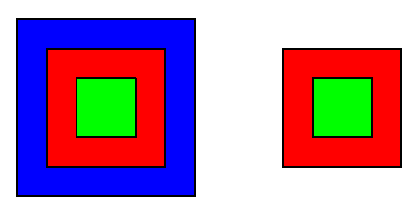
\includegraphics[width=0.5\textwidth]{sample3}
  \caption{A possible solution to sample 3.
  On the left, a green box is placed inside a red box which is placed inside a blue box.
  On the right, a green box is placed inside a red box.}
  \label{fig:sample3}
\end{figure}

Can you determine in what order to visit the stores to minimize the number of \emph{outer boxes} (i.e.\ boxes that are not inside another box), if you place the boxes optimally?

\section*{Input}
The input starts with the number $N$, the number of boxes, where $1\le N \le 1\,000$. Then follow $N$ lines with side length
$l_i$ ($1 \le l_i \le 10\,000\,000$) and color $f_i$ (R, G, or B) for each box.

\section*{Output}
You shall output two lines.
The first line shall contain the order you visit the stores in, in the form $f_1\text{ }f_2\text{ }f_3$.
The second line shall consist of one integer --- the minimum number of outer boxes you can achieve after placing boxes inside each other.

If multiple orders give the same minimum number of outer boxes, you may output any of these orders.

\section*{Scoring}
Your solution will be tested on a set of test groups. To earn points for a group, you must pass all test cases in that group.

\noindent
\begin{tabular}{| l | l | l |}
\hline
Group & Points & Constraints \\ \hline
1     & 50         & You will always visit the stores in the order \texttt{B G R} \\ \hline
2     & 50         & No additional constraints. \\ \hline
\end{tabular}

\section*{Explanation of Sample 3}
A possible solution is illustrated in Figure~\ref{fig:sample3}.
The optimal order is to visit the stores in the order blue, red, green.

We can then place the two G boxes (size 1) inside one R box (size 10) each.
After that, one of the R boxes can be placed inside a B box.
This leaves one R box and one B box as outer boxes.
